\documentclass[aspectratio=169,9pt]{beamer}

\usetheme{Madrid}
\usecolortheme{default}
\usefonttheme{professionalfonts}
\usepackage{graphicx}
\usepackage{booktabs}
\usepackage{array}
\usepackage{tikz}
\usepackage{hyperref}
\usepackage{xcolor}
\usetikzlibrary{positioning,arrows.meta,calc}

\definecolor{cvblue}{RGB}{18,54,92}
\definecolor{cvcyan}{RGB}{32,120,150}
\definecolor{cvorange}{RGB}{205,112,36}
\definecolor{cvgreen}{RGB}{68,130,88}
\definecolor{cvgray}{RGB}{70,78,86}
\definecolor{cvlight}{RGB}{242,246,250}

\setbeamercolor{palette primary}{bg=cvblue,fg=white}
\setbeamercolor{palette secondary}{bg=cvblue,fg=white}
\setbeamercolor{palette tertiary}{bg=cvblue,fg=white}
\setbeamercolor{frametitle}{bg=cvblue,fg=white}
\setbeamercolor{title}{fg=cvblue}
\setbeamercolor{block title}{bg=cvblue,fg=white}
\setbeamercolor{block body}{bg=cvlight,fg=black}
\setbeamertemplate{navigation symbols}{}
\setbeamertemplate{footline}[frame number]

\tikzset{
  box/.style={draw, rounded corners, fill=cvlight, align=center, minimum height=0.68cm, font=\scriptsize},
  smallbox/.style={draw, rounded corners, fill=cvlight, align=center, minimum height=0.52cm, font=\tiny},
  arrow/.style={-{Latex[length=2mm]}, thick, cvblue},
  mod/.style={draw, rounded corners, fill=cvorange!15, align=center, font=\scriptsize},
  outbox/.style={draw, rounded corners, fill=cvgreen!15, align=center, font=\scriptsize}
}

\title[CV Assignment 2]{From Images to Decisions: A Reproducible CV Study Across Classification, Segmentation, and Aerial Detection}
\author[Yuheng Li]{\texorpdfstring{Yuheng Li\\Student ID: 23307130334}{Yuheng Li, Student ID: 23307130334}}
\institute{GitHub: \href{https://github.com/yuheng-li-ai/CV_Midterm}{CV\_Midterm}\\ModelScope: \href{https://www.modelscope.cn/models/yuhengli/cv-hw2-final-model}{cv-hw2-final-model}}
\date{CV Assignment 2 Presentation}

\begin{document}

\begin{frame}
  \titlepage
\end{frame}

\begin{frame}{What This Presentation Explains}
  \begin{columns}[T]
    \begin{column}{0.32\textwidth}
      \begin{block}{Classification}
        How an RGB pet image becomes a 37-class breed prediction.
      \end{block}
    \end{column}
    \begin{column}{0.32\textwidth}
      \begin{block}{Segmentation}
        How a pixel mask is produced and optimized with CE/Dice/Focal losses.
      \end{block}
    \end{column}
    \begin{column}{0.32\textwidth}
      \begin{block}{Detection + Tracking}
        How VisDrone boxes become YOLO predictions, object IDs, and line counts.
      \end{block}
    \end{column}
  \end{columns}
  \vspace{0.7em}
  \begin{block}{Thesis}
    Each extension is evaluated by asking: where is the bottleneck, what exactly was modified, and did the modification match the bottleneck?
  \end{block}
\end{frame}

\begin{frame}{Final Results First}
  \begin{table}
    \centering
    \small
    \begin{tabular}{llll}
      \toprule
      Task & Final model & Selection metric & Final result\\
      \midrule
      Classification & ImageNet ResNet-34 & validation accuracy & \textbf{90.60\% test accuracy}\\
      Segmentation & U-Net + Dice loss & validation mIoU & \textbf{77.90\% test mIoU}\\
      Detection & YOLO11m, img size 960 & validation mAP50-95 & \textbf{0.5356 mAP50 / 0.3310 mAP50-95}\\
      Tracking & YOLO11m + ByteTrack & qualitative stability & line-crossing video analysis\\
      \bottomrule
    \end{tabular}
  \end{table}
  \begin{block}{Interpretation}
    The best gains came from pretrained representation, overlap-aware segmentation loss, and high-resolution dense detection.
  \end{block}
\end{frame}

\begin{frame}{Harness: Experimental Control, Not Decoration}
  \centering
  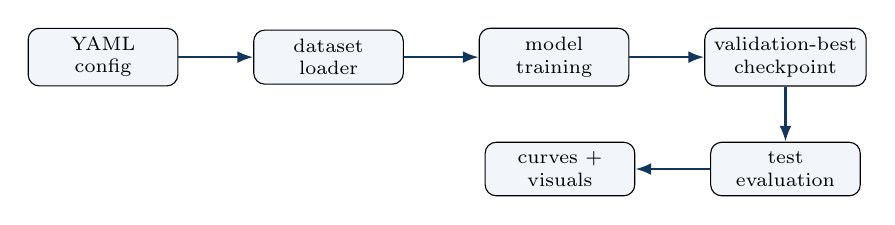
\begin{tikzpicture}[node distance=0.95cm]
    \node[box, minimum width=1.9cm] (cfg) {YAML\\config};
    \node[box, minimum width=1.9cm, right=of cfg] (data) {dataset\\loader};
    \node[box, minimum width=1.9cm, right=of data] (train) {model\\training};
    \node[box, minimum width=1.9cm, right=of train] (best) {validation-best\\checkpoint};
    \node[box, minimum width=1.9cm, below=0.7cm of best] (eval) {test\\evaluation};
    \node[box, minimum width=1.9cm, left=of eval] (vis) {curves +\\visuals};
    \draw[arrow] (cfg) -- (data);
    \draw[arrow] (data) -- (train);
    \draw[arrow] (train) -- (best);
    \draw[arrow] (best) -- (eval);
    \draw[arrow] (eval) -- (vis);
  \end{tikzpicture}
  \vspace{0.8em}
  \begin{itemize}
    \item Classification selects by validation accuracy; segmentation by validation mIoU; detection by validation mAP50-95.
    \item The test result is computed from the selected checkpoint, not from the last epoch.
  \end{itemize}
\end{frame}

\begin{frame}{Classification Data Flow}
  \centering
  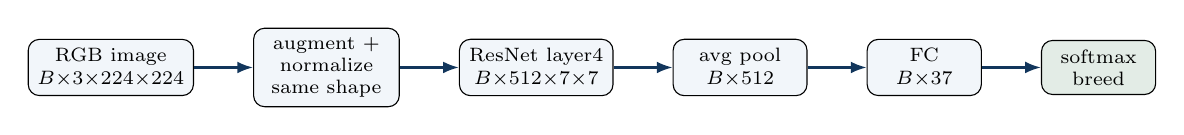
\begin{tikzpicture}[node distance=0.75cm]
    \node[box, minimum width=1.8cm] (img) {RGB image\\$B{\times}3{\times}224{\times}224$};
    \node[box, minimum width=1.85cm, right=of img] (tf) {augment +\\normalize\\same shape};
    \node[box, minimum width=1.95cm, right=of tf] (res) {ResNet layer4\\$B{\times}512{\times}7{\times}7$};
    \node[box, minimum width=1.7cm, right=of res] (pool) {avg pool\\$B{\times}512$};
    \node[box, minimum width=1.45cm, right=of pool] (fc) {FC\\$B{\times}37$};
    \node[outbox, minimum width=1.45cm, right=of fc] (pred) {softmax\\breed};
    \draw[arrow] (img) -- (tf);
    \draw[arrow] (tf) -- (res);
    \draw[arrow] (res) -- (pool);
    \draw[arrow] (pool) -- (fc);
    \draw[arrow] (fc) -- (pred);
  \end{tikzpicture}
  \vspace{0.8em}
  \begin{block}{Training signal}
    Cross entropy compares the 37 logits with the category label. Accuracy is the fraction of images whose top-1 logit matches the ground-truth class.
  \end{block}
\end{frame}

\begin{frame}{ResNet Baseline Architecture From Code}
  \begin{columns}[T]
    \begin{column}{0.58\textwidth}
      \centering
      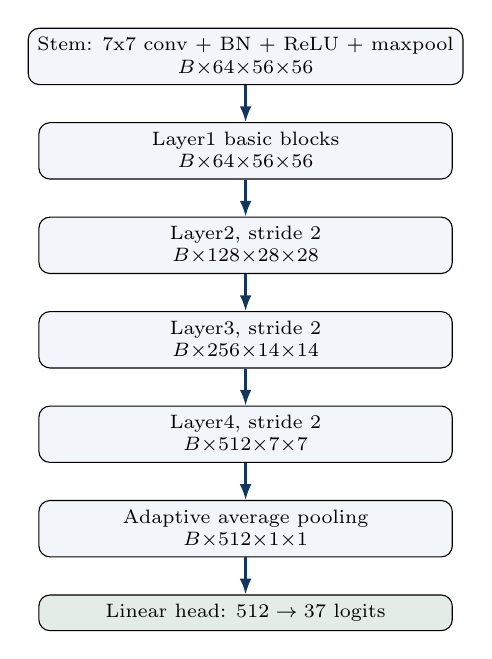
\begin{tikzpicture}[node distance=0.47cm]
        \node[box, minimum width=5.25cm] (stem) {Stem: 7x7 conv + BN + ReLU + maxpool\\$B{\times}64{\times}56{\times}56$};
        \node[box, minimum width=5.25cm, below=of stem] (l1) {Layer1 basic blocks\\$B{\times}64{\times}56{\times}56$};
        \node[box, minimum width=5.25cm, below=of l1] (l2) {Layer2, stride 2\\$B{\times}128{\times}28{\times}28$};
        \node[box, minimum width=5.25cm, below=of l2] (l3) {Layer3, stride 2\\$B{\times}256{\times}14{\times}14$};
        \node[box, minimum width=5.25cm, below=of l3] (l4) {Layer4, stride 2\\$B{\times}512{\times}7{\times}7$};
        \node[box, minimum width=5.25cm, below=of l4] (avg) {Adaptive average pooling\\$B{\times}512{\times}1{\times}1$};
        \node[outbox, minimum width=5.25cm, below=of avg] (head) {Linear head: $512 \rightarrow 37$ logits};
        \foreach \a/\b in {stem/l1,l1/l2,l2/l3,l3/l4,l4/avg,avg/head}{\draw[arrow] (\a) -- (\b);}
      \end{tikzpicture}
    \end{column}
    \begin{column}{0.38\textwidth}
      \begin{block}{Baseline modification}
        Start from torchvision ResNet-18. Replace only the original ImageNet FC layer with a new 37-class FC layer.
      \end{block}
      \begin{block}{ResNet-18 vs 34}
        Spatial dimensions stay the same. ResNet-34 only uses more basic blocks: $[3,4,6,3]$ instead of $[2,2,2,2]$.
      \end{block}
      \begin{block}{Optimization}
        Backbone LR = $10^{-4}$; head LR = $10^{-3}$. The new head is allowed to adapt faster.
      \end{block}
    \end{column}
  \end{columns}
\end{frame}

\begin{frame}{Classification Extensions: Where They Enter}
  \small
  \begin{tabular}{p{0.2\textwidth}p{0.36\textwidth}p{0.34\textwidth}}
    \toprule
    Extension & Exact change & Difference from baseline\\
    \midrule
    Random init & Use ResNet-18 with \texttt{weights=None}. & Same architecture, no ImageNet features.\\
    ResNet-34 & Replace ResNet-18 backbone with pretrained ResNet-34. & Deeper residual backbone, same 37-class head.\\
    Label smoothing & Set \texttt{label\_smoothing=0.1} in CrossEntropyLoss. & Target is softened instead of one-hot.\\
    Freeze-unfreeze & Freeze backbone for first 3 epochs, then unfreeze all layers. & Early training updates only head parameters.\\
    \bottomrule
  \end{tabular}
  \vspace{0.7em}
  \begin{block}{Common rule}
    Dataset, transforms, optimizer family, and validation-best selection stay fixed.
  \end{block}
\end{frame}

\begin{frame}{Classification Hyperparameter Grid Search}
  \begin{columns}[T]
    \begin{column}{0.56\textwidth}
      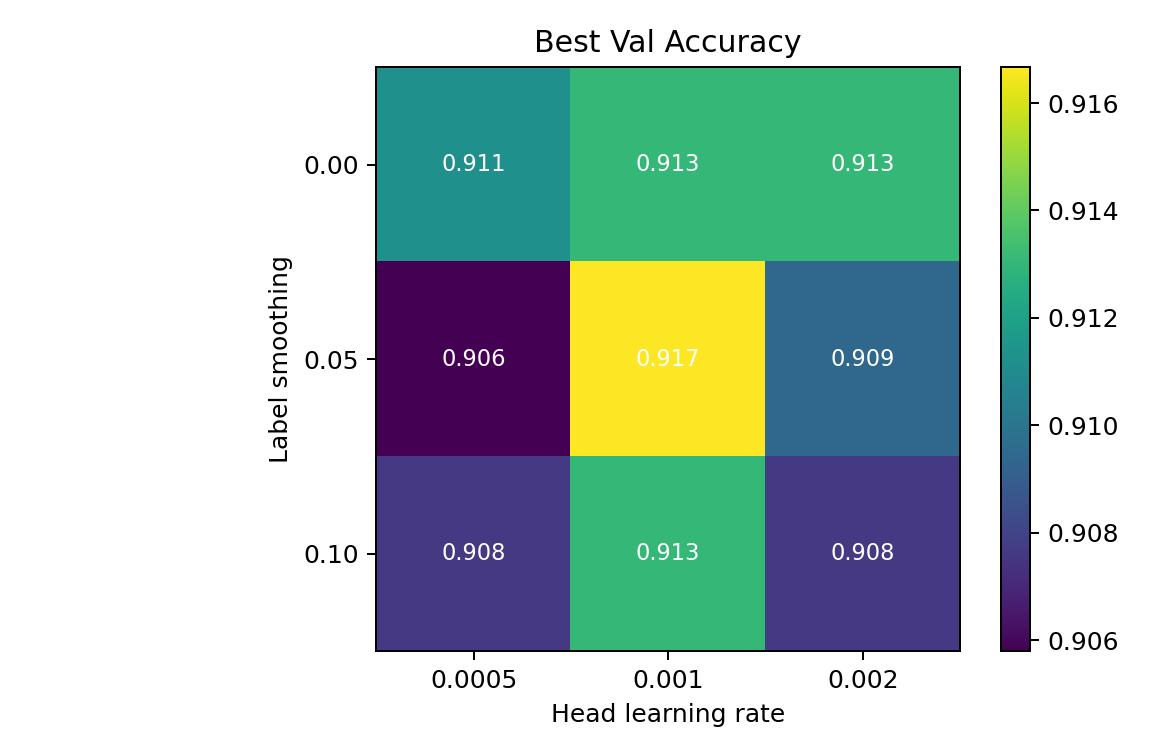
\includegraphics[width=\textwidth]{assets/classification_hparam_val_heatmap.png}
    \end{column}
    \begin{column}{0.39\textwidth}
      \begin{block}{Controlled grid}
        Fixed pretrained ResNet-18, batch 32, image size 224, backbone LR $10^{-4}$, weight decay $10^{-4}$.
      \end{block}
      \begin{block}{Swept hyperparameters}
        \small
        \texttt{label\_smoothing}: 0, 0.05, 0.10.\\
        \texttt{head\_lr}: $5{\times}10^{-4}$, $10^{-3}$, $2{\times}10^{-3}$.
      \end{block}
      \begin{block}{Reading}
        Best validation setting is label smoothing 0.05 and head LR $10^{-3}$, but gains are small.
      \end{block}
    \end{column}
  \end{columns}
\end{frame}

\begin{frame}{SE Block: The Attention Extension}
  \begin{columns}[T]
    \begin{column}{0.56\textwidth}
      \centering
      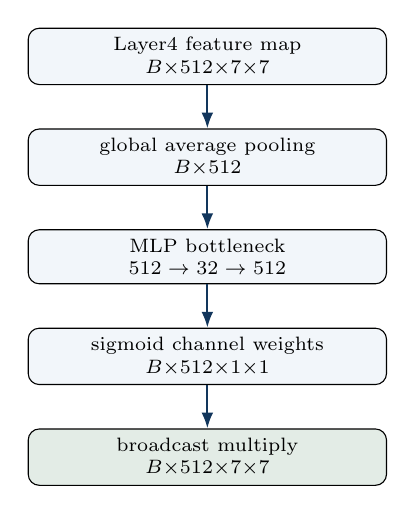
\begin{tikzpicture}[node distance=0.55cm]
        \node[box, minimum width=4.55cm] (feat) {Layer4 feature map\\$B{\times}512{\times}7{\times}7$};
        \node[box, minimum width=4.55cm, below=of feat] (gap) {global average pooling\\$B{\times}512$};
        \node[box, minimum width=4.55cm, below=of gap] (mlp) {MLP bottleneck\\$512 \rightarrow 32 \rightarrow 512$};
        \node[box, minimum width=4.55cm, below=of mlp] (sig) {sigmoid channel weights\\$B{\times}512{\times}1{\times}1$};
        \node[outbox, minimum width=4.55cm, below=of sig] (mul) {broadcast multiply\\$B{\times}512{\times}7{\times}7$};
        \foreach \a/\b in {feat/gap,gap/mlp,mlp/sig,sig/mul}{\draw[arrow] (\a) -- (\b);}
      \end{tikzpicture}
    \end{column}
    \begin{column}{0.4\textwidth}
      \begin{block}{Insertion point}
        In code, SE is inserted after ResNet layer4 and before average pooling.
      \end{block}
      \begin{block}{Purpose}
        It learns which channels should be emphasized for fine-grained breed cues.
      \end{block}
      \begin{block}{Result}
        It did not beat the pretrained ResNet-18 baseline, so the added module was not automatically useful.
      \end{block}
    \end{column}
  \end{columns}
\end{frame}

\begin{frame}{Classification Results}
  \begin{columns}[T]
    \begin{column}{0.6\textwidth}
      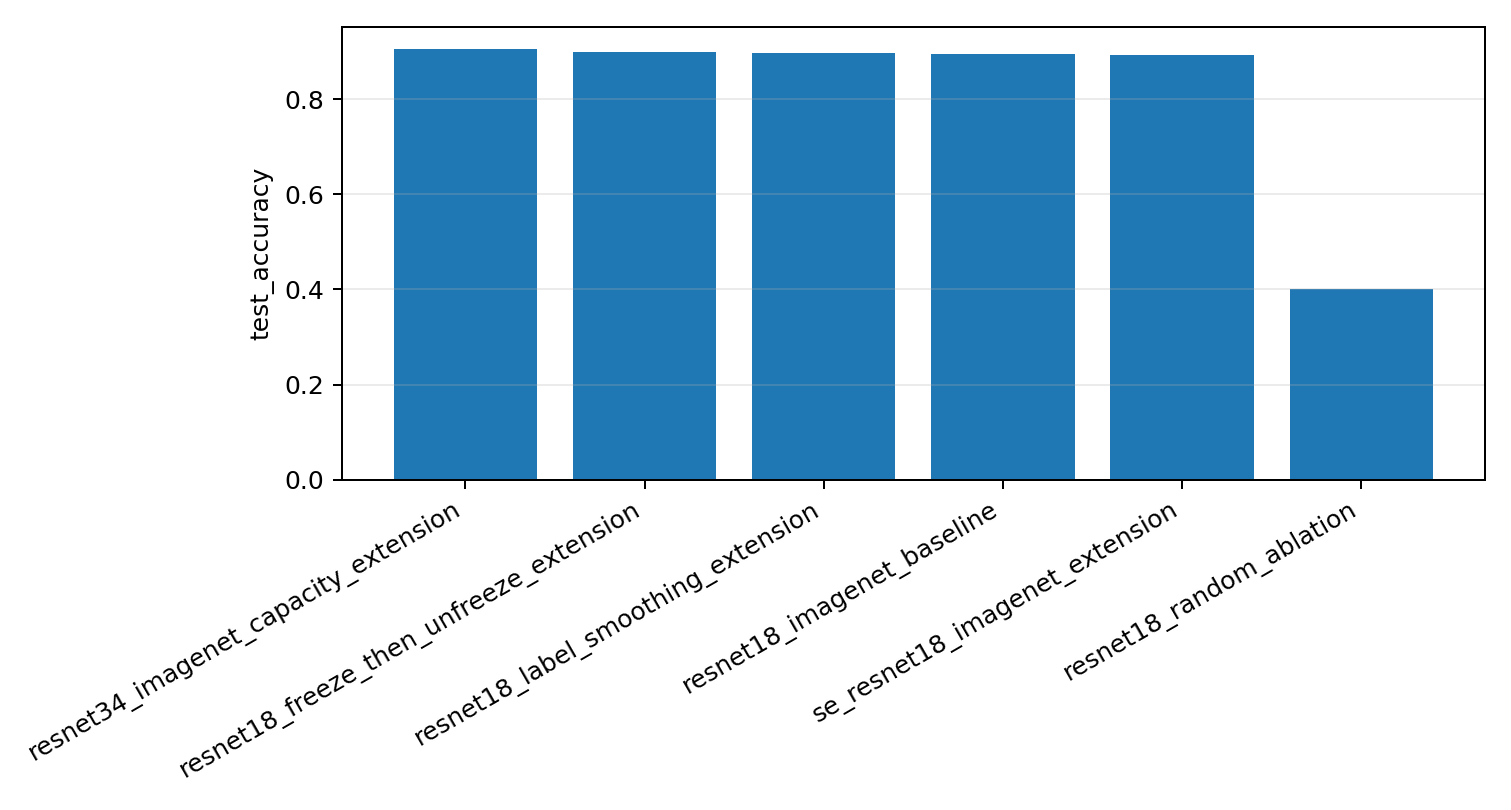
\includegraphics[width=\textwidth]{assets/classification_test_accuracy.png}
    \end{column}
    \begin{column}{0.36\textwidth}
      \begin{block}{Key evidence}
        \begin{itemize}
          \item Random ResNet-18: \textbf{40.15\%}.
          \item Pretrained ResNet-18: \textbf{89.40\%}.
          \item Pretrained ResNet-34: \textbf{90.60\%}.
        \end{itemize}
      \end{block}
      \begin{block}{Reading}
        Transfer learning is the largest factor; extra capacity gives the best extension.
      \end{block}
    \end{column}
  \end{columns}
\end{frame}

\begin{frame}{Classification Failure Cases}
  \begin{columns}[T]
    \begin{column}{0.45\textwidth}
      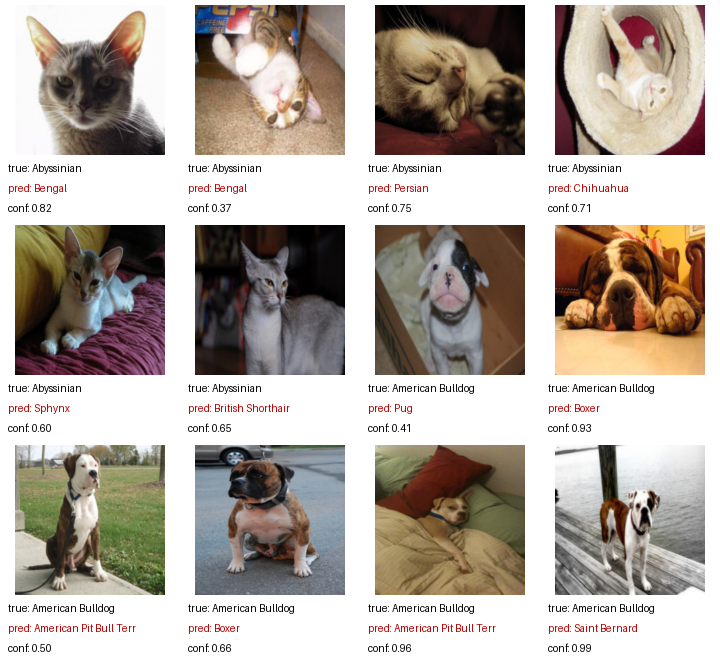
\includegraphics[width=\textwidth]{assets/classification_mistakes_top12.png}
    \end{column}
    \begin{column}{0.5\textwidth}
      \begin{block}{What the mistakes mean}
        The model usually fails between visually similar breeds, not between unrelated categories.
      \end{block}
      \begin{itemize}
        \item Terrier/bulldog-like breeds share short fur and head structure.
        \item Ragdoll/Birman-like cats share color masks and coat patterns.
        \item This explains why representation capacity helps but does not remove all errors.
      \end{itemize}
    \end{column}
  \end{columns}
\end{frame}

\begin{frame}{Segmentation Data Flow}
  \centering
  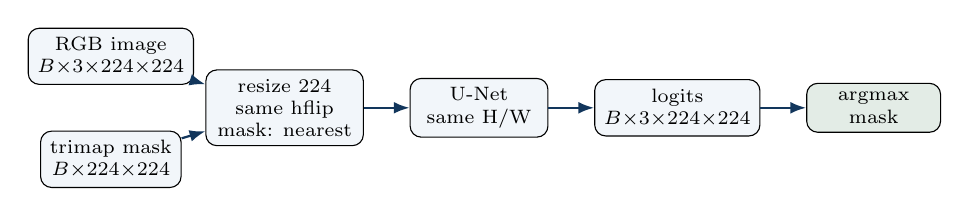
\begin{tikzpicture}[node distance=0.58cm]
    \node[box, minimum width=1.75cm] (img) {RGB image\\$B{\times}3{\times}224{\times}224$};
    \node[box, minimum width=1.75cm, below=of img] (mask) {trimap mask\\$B{\times}224{\times}224$};
    \node[box, minimum width=2.0cm, right=1.2cm of $(img)!0.5!(mask)$] (tf) {resize 224\\same hflip\\mask: nearest};
    \node[box, minimum width=1.75cm, right=of tf] (unet) {U-Net\\same H/W};
    \node[box, minimum width=1.8cm, right=of unet] (logits) {logits\\$B{\times}3{\times}224{\times}224$};
    \node[outbox, minimum width=1.7cm, right=of logits] (argmax) {argmax\\mask};
    \draw[arrow] (img) -- (tf);
    \draw[arrow] (mask) -- (tf);
    \draw[arrow] (tf) -- (unet);
    \draw[arrow] (unet) -- (logits);
    \draw[arrow] (logits) -- (argmax);
  \end{tikzpicture}
  \vspace{0.7em}
  \begin{block}{Code-level detail}
    The original trimap values are clipped to 1--3 and shifted to 0--2. Thus the model predicts three classes: foreground, boundary, and background.
  \end{block}
\end{frame}

\begin{frame}{U-Net Architecture From Code}
  \centering
  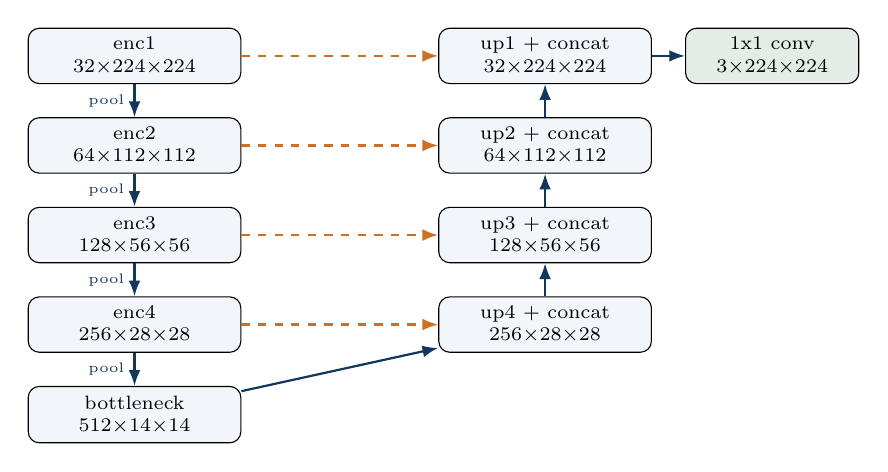
\begin{tikzpicture}[node distance=0.42cm]
    \node[box, minimum width=2.7cm] (e1) {enc1\\$32{\times}224{\times}224$};
    \node[box, minimum width=2.7cm, below=of e1] (e2) {enc2\\$64{\times}112{\times}112$};
    \node[box, minimum width=2.7cm, below=of e2] (e3) {enc3\\$128{\times}56{\times}56$};
    \node[box, minimum width=2.7cm, below=of e3] (e4) {enc4\\$256{\times}28{\times}28$};
    \node[box, minimum width=2.7cm, below=of e4] (b) {bottleneck\\$512{\times}14{\times}14$};
    \node[box, minimum width=2.7cm, right=2.5cm of e4] (d4) {up4 + concat\\$256{\times}28{\times}28$};
    \node[box, minimum width=2.7cm, right=2.5cm of e3] (d3) {up3 + concat\\$128{\times}56{\times}56$};
    \node[box, minimum width=2.7cm, right=2.5cm of e2] (d2) {up2 + concat\\$64{\times}112{\times}112$};
    \node[box, minimum width=2.7cm, right=2.5cm of e1] (d1) {up1 + concat\\$32{\times}224{\times}224$};
    \node[outbox, minimum width=2.2cm, right=of d1] (head) {1x1 conv\\$3{\times}224{\times}224$};
    \foreach \a/\b in {e1/e2,e2/e3,e3/e4,e4/b}{\draw[arrow] (\a) -- node[left,font=\tiny]{pool} (\b);}
    \draw[arrow] (b) -- (d4);
    \draw[arrow] (d4) -- (d3);
    \draw[arrow] (d3) -- (d2);
    \draw[arrow] (d2) -- (d1);
    \draw[arrow] (d1) -- (head);
    \draw[arrow, dashed, cvorange] (e4.east) -- (d4.west);
    \draw[arrow, dashed, cvorange] (e3.east) -- (d3.west);
    \draw[arrow, dashed, cvorange] (e2.east) -- (d2.west);
    \draw[arrow, dashed, cvorange] (e1.east) -- (d1.west);
  \end{tikzpicture}
  \par\vspace{0.4em}
  {\scriptsize Each DoubleConv is Conv-BN-ReLU-Conv-BN-ReLU. Dashed arrows are skip concatenations.}
\end{frame}

\begin{frame}{How the Segmentation Losses Are Applied}
  \begin{columns}[T]
    \begin{column}{0.33\textwidth}
      \begin{block}{Cross-Entropy}
        Uses raw 3-channel logits and integer mask labels. Each pixel is treated as a 3-way classification problem.
      \end{block}
    \end{column}
    \begin{column}{0.33\textwidth}
      \begin{block}{Dice}
        Applies softmax to logits, converts target to a one-hot mask, then computes overlap:
        \[
        1-\frac{2|P\cap Y|+s}{|P|+|Y|+s}
        \]
      \end{block}
    \end{column}
    \begin{column}{0.33\textwidth}
      \begin{block}{CE + Dice}
        Adds the two losses. CE stabilizes pixel classification; Dice aligns with region overlap and mIoU.
      \end{block}
    \end{column}
  \end{columns}
\end{frame}

\begin{frame}{Segmentation Extensions: Loss-Level Changes}
  \centering
  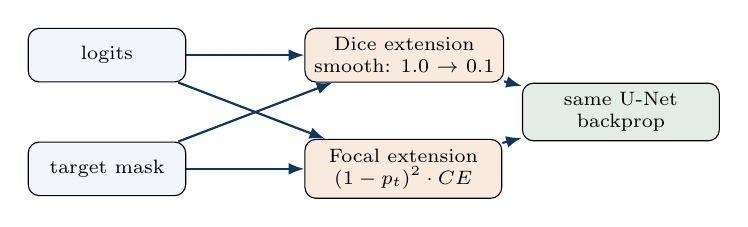
\begin{tikzpicture}[node distance=0.75cm]
    \node[box, minimum width=2.0cm] (logits) {logits};
    \node[box, minimum width=2.0cm, below=of logits] (target) {target mask};
    \node[mod, minimum width=2.5cm, right=1.5cm of logits] (dice) {Dice extension\\smooth: 1.0 $\rightarrow$ 0.1};
    \node[mod, minimum width=2.5cm, right=1.5cm of target] (focal) {Focal extension\\$(1-p_t)^2 \cdot CE$};
    \node[outbox, minimum width=2.5cm, right=1.5cm of $(dice)!0.5!(focal)$] (back) {same U-Net\\backprop};
    \draw[arrow] (logits) -- (dice);
    \draw[arrow] (target) -- (dice);
    \draw[arrow] (logits) -- (focal);
    \draw[arrow] (target) -- (focal);
    \draw[arrow] (dice) -- (back);
    \draw[arrow] (focal) -- (back);
  \end{tikzpicture}
  \vspace{0.8em}
  \begin{block}{Important control}
    The architecture, image size, optimizer, and 60-epoch budget are unchanged; only the criterion changes.
  \end{block}
\end{frame}

\begin{frame}{Segmentation Results}
  \begin{columns}[T]
    \begin{column}{0.53\textwidth}
      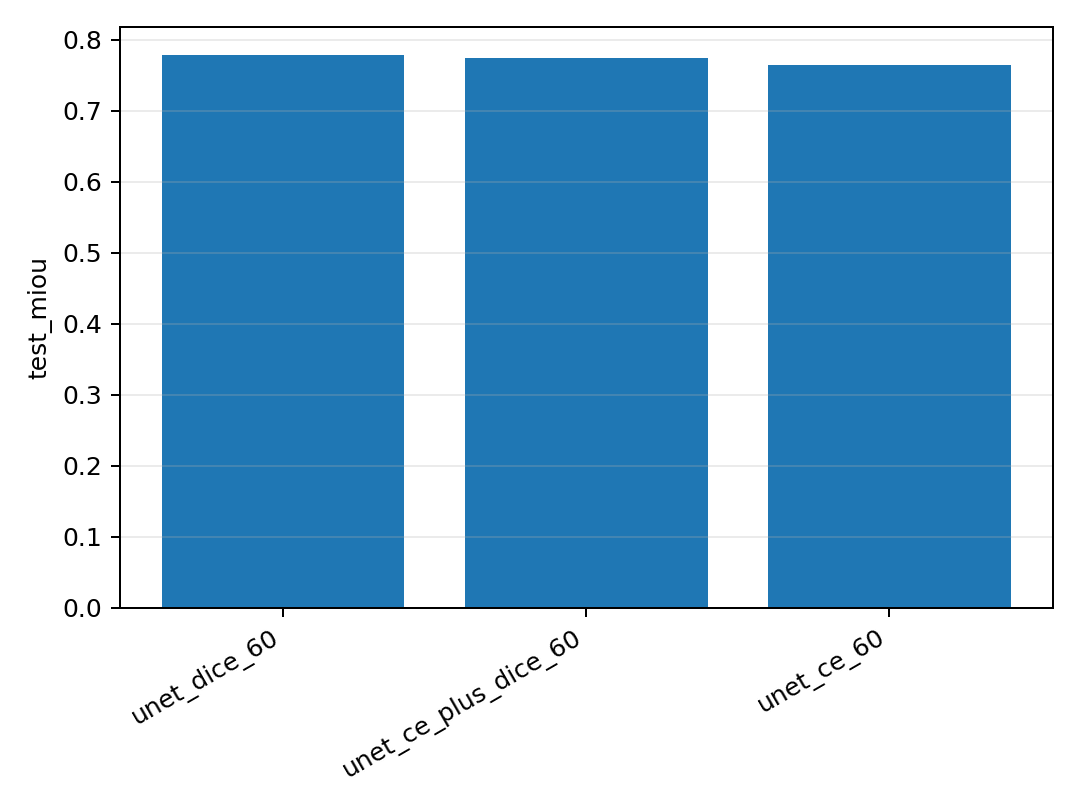
\includegraphics[width=\textwidth]{assets/segmentation_test_miou.png}
    \end{column}
    \begin{column}{0.43\textwidth}
      \begin{block}{Required comparison}
        CE: 76.40\%; Dice: \textbf{77.90\%}; CE+Dice: 77.41\%.
      \end{block}
      \begin{block}{Extensions}
        Dice smooth 0.1: 77.85\%; Focal: 76.45\%.
      \end{block}
      \begin{block}{Reading}
        Dice is best because the evaluation metric is overlap-based.
      \end{block}
    \end{column}
  \end{columns}
\end{frame}

\begin{frame}{Segmentation Qualitative Explanation}
  \begin{columns}[T]
    \begin{column}{0.48\textwidth}
      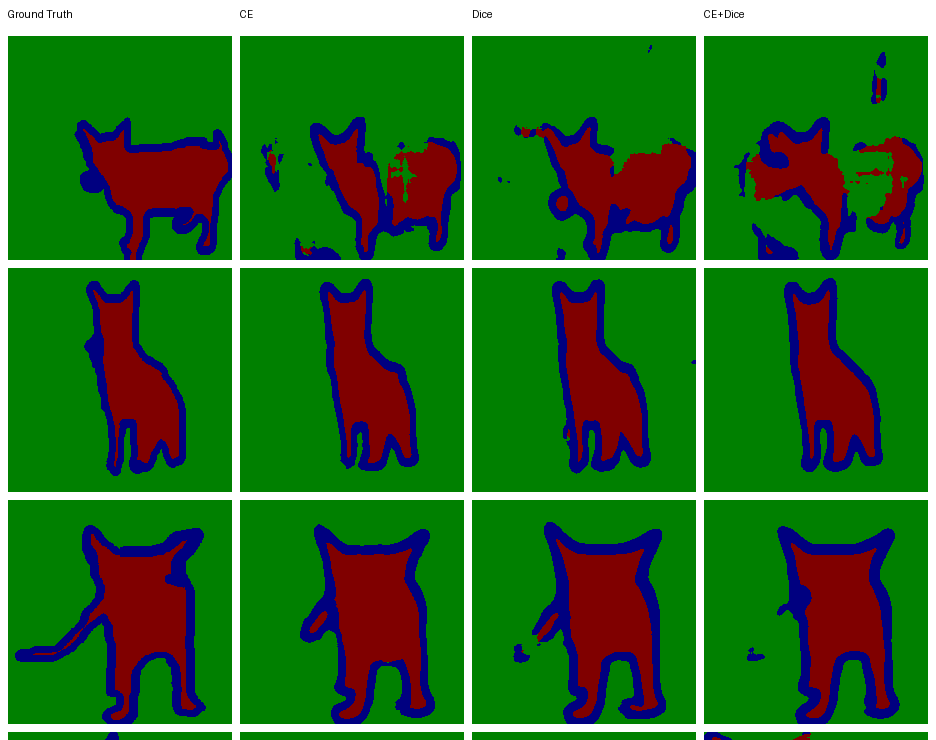
\includegraphics[width=\textwidth,height=0.25\textheight,keepaspectratio]{assets/segmentation_required_masks_compact.png}
      \vspace{0.4em}
      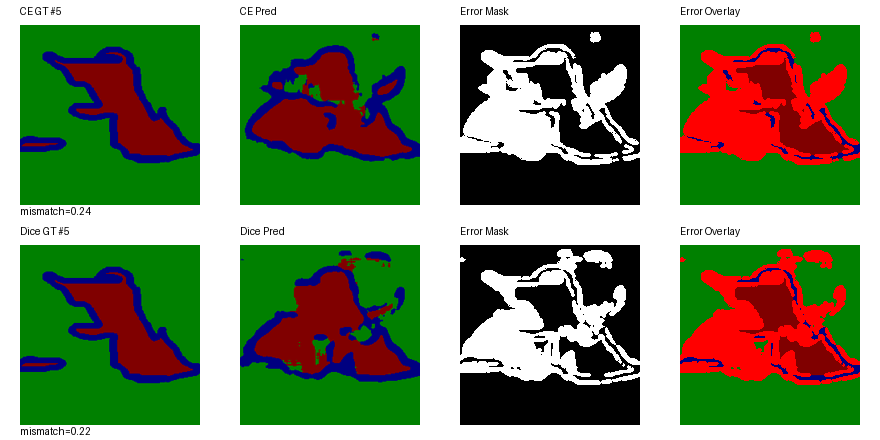
\includegraphics[width=\textwidth,height=0.25\textheight,keepaspectratio]{assets/segmentation_error_cases_compact.png}
    \end{column}
    \begin{column}{0.48\textwidth}
      \begin{block}{What remains hard}
        The coarse pet region is usually correct, but boundary pixels remain unstable.
      \end{block}
      \begin{itemize}
        \item Thin legs, ears, and fur edges are hard.
        \item Low-contrast foreground/background regions are ambiguous.
        \item This explains why Focal Loss does not automatically improve mIoU.
      \end{itemize}
    \end{column}
  \end{columns}
\end{frame}

\begin{frame}{VisDrone Label Conversion}
  \centering
  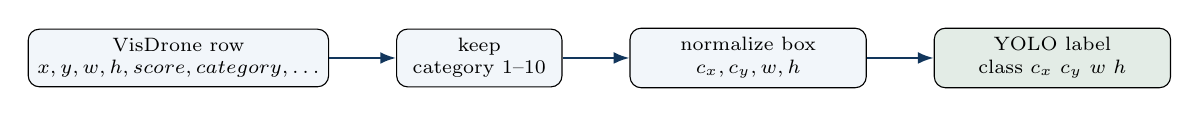
\begin{tikzpicture}[node distance=0.85cm]
    \node[box, minimum width=3.1cm] (raw) {VisDrone row\\$x,y,w,h,score,category,\dots$};
    \node[box, minimum width=2.1cm, right=of raw] (filter) {keep\\category 1--10};
    \node[box, minimum width=3.0cm, right=of filter] (norm) {normalize box\\$c_x,c_y,w,h$};
    \node[outbox, minimum width=3.0cm, right=of norm] (yolo) {YOLO label\\class $c_x$ $c_y$ $w$ $h$};
    \draw[arrow] (raw) -- (filter);
    \draw[arrow] (filter) -- (norm);
    \draw[arrow] (norm) -- (yolo);
  \end{tikzpicture}
  \vspace{0.8em}
  \begin{block}{Dataset output}
    The converter creates symlinked image folders, YOLO-format label files, and a \texttt{visdrone.yaml} file with 10 classes.
  \end{block}
\end{frame}

\begin{frame}{YOLO Detection Training Pipeline}
  \centering
  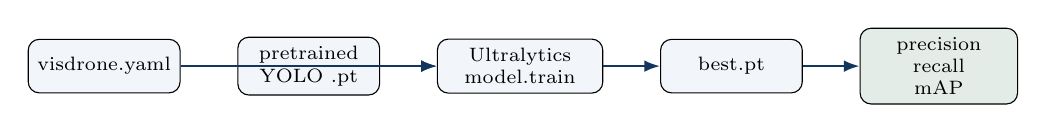
\begin{tikzpicture}[node distance=0.72cm]
    \node[box, minimum width=1.8cm] (yaml) {visdrone.yaml};
    \node[box, minimum width=1.8cm, right=of yaml] (pt) {pretrained\\YOLO .pt};
    \node[box, minimum width=2.1cm, right=of pt] (train) {Ultralytics\\model.train};
    \node[box, minimum width=1.8cm, right=of train] (best) {best.pt};
    \node[outbox, minimum width=2.0cm, right=of best] (metrics) {precision\\recall\\mAP};
    \draw[arrow] (yaml) -- (train);
    \draw[arrow] (pt) -- (train);
    \draw[arrow] (train) -- (best);
    \draw[arrow] (best) -- (metrics);
  \end{tikzpicture}
  \vspace{0.8em}
  \begin{itemize}
    \item Baseline: YOLOv8n, image size 640.
    \item Capacity extension: YOLOv8s, same data and same image size.
    \item Strong extension: YOLO11m with image size 960.
  \end{itemize}
\end{frame}

\begin{frame}{YOLOv8n vs YOLOv8s vs YOLO11m}
  \begin{columns}[T]
    \begin{column}{0.66\textwidth}
      \begin{table}
        \centering
        \scriptsize
        \begin{tabular}{lccc}
          \toprule
          Model & Main blocks & Scale / size & Parameters\\
          \midrule
          YOLOv8n & C2f + SPPF + Detect & width 0.25 & 3.16M\\
          YOLOv8s & C2f + SPPF + Detect & width 0.50 & 11.17M\\
          YOLO11m & C3k2 + SPPF + C2PSA + Detect & scale m & 20.11M\\
          \bottomrule
        \end{tabular}
      \end{table}
      \vspace{0.3em}
      \begin{table}
        \centering
        \scriptsize
        \begin{tabular}{lccc}
          \toprule
          Model & imgsz & mAP50 & mAP50-95\\
          \midrule
          YOLOv8n & 640 & 0.2985 & 0.1665\\
          YOLOv8s & 640 & 0.3819 & 0.2211\\
          YOLO11m & 960 & \textbf{0.5356} & \textbf{0.3310}\\
          \bottomrule
        \end{tabular}
      \end{table}
    \end{column}
    \begin{column}{0.30\textwidth}
      \begin{block}{Controlled read}
        v8n $\rightarrow$ v8s keeps 640 input, so the gain mainly reflects detector capacity.
      \end{block}
      \begin{block}{Practical read}
        YOLO11m@960 changes both model family and resolution, so it is a stronger practical detector rather than a single-factor ablation.
      \end{block}
    \end{column}
  \end{columns}
\end{frame}

\begin{frame}{YOLO11m Architecture: More Detailed View}
  \begin{columns}[T]
    \begin{column}{0.62\textwidth}
      \centering
      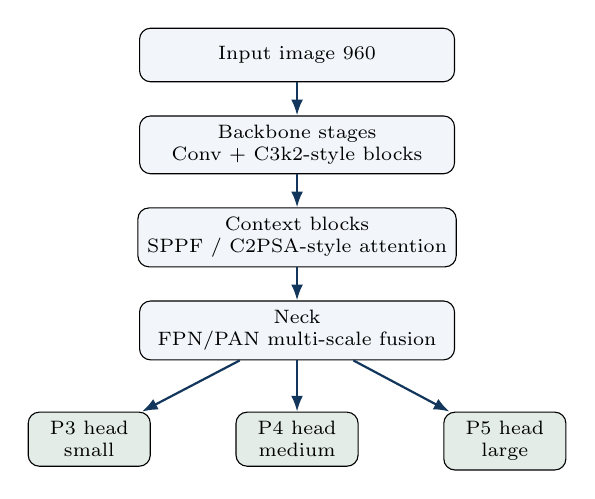
\begin{tikzpicture}[node distance=0.42cm]
        \node[box, minimum width=4.0cm] (in) {Input image 960};
        \node[box, minimum width=4.0cm, below=of in] (s1) {Backbone stages\\Conv + C3k2-style blocks};
        \node[box, minimum width=4.0cm, below=of s1] (ctx) {Context blocks\\SPPF / C2PSA-style attention};
        \node[box, minimum width=4.0cm, below=of ctx] (neck) {Neck\\FPN/PAN multi-scale fusion};
        \node[outbox, minimum width=1.55cm, below left=0.65cm and -0.15cm of neck] (p3) {P3 head\\small};
        \node[outbox, minimum width=1.55cm, below=0.65cm of neck] (p4) {P4 head\\medium};
        \node[outbox, minimum width=1.55cm, below right=0.65cm and -0.15cm of neck] (p5) {P5 head\\large};
        \draw[arrow] (in) -- (s1);
        \draw[arrow] (s1) -- (ctx);
        \draw[arrow] (ctx) -- (neck);
        \draw[arrow] (neck) -- (p3);
        \draw[arrow] (neck) -- (p4);
        \draw[arrow] (neck) -- (p5);
      \end{tikzpicture}
    \end{column}
    \begin{column}{0.34\textwidth}
      \begin{block}{What I changed}
        I did not edit YOLO11m internals. I selected YOLO11m and increased input size to 960.
      \end{block}
      \begin{block}{Why for VisDrone}
        Small objects occupy more pixels at 960 input, and multi-scale heads help dense objects at different sizes.
      \end{block}
      {\tiny Source: Ultralytics YOLO11 docs, \url{https://docs.ultralytics.com/models/yolo11/}}
    \end{column}
  \end{columns}
\end{frame}

\begin{frame}{Detection Extensions: What Changed}
  \small
  \begin{tabular}{p{0.22\textwidth}p{0.35\textwidth}p{0.33\textwidth}}
    \toprule
    Experiment & Exact modification & What it tests\\
    \midrule
    YOLOv8n baseline & \texttt{model=yolov8n.pt}, \texttt{imgsz=640}. & Lightweight single-stage baseline.\\
    YOLOv8s & Change only model size to \texttt{yolov8s.pt}; keep \texttt{imgsz=640}. & Whether more capacity helps.\\
    YOLO11m@960 & Change model to \texttt{yolo11m.pt}; increase \texttt{imgsz=960}. & Practical combination of newer capacity and higher small-object resolution.\\
    \bottomrule
  \end{tabular}
  \vspace{0.7em}
  \begin{block}{Limitation}
    YOLO11m and 960 resolution are not fully disentangled, so the conclusion is about this practical combined extension.
  \end{block}
\end{frame}

\begin{frame}{Detection Results}
  \begin{columns}[T]
    \begin{column}{0.46\textwidth}
      \begin{table}
        \centering
        \small
        \begin{tabular}{lccc}
          \toprule
          Model & Size & mAP50 & mAP50-95\\
          \midrule
          YOLOv8n & 640 & 0.2985 & 0.1665\\
          YOLOv8s & 640 & 0.3819 & 0.2211\\
          YOLO11m & 960 & \textbf{0.5356} & \textbf{0.3310}\\
          \bottomrule
        \end{tabular}
      \end{table}
      \begin{block}{Reading}
        VisDrone benefits strongly from larger capacity and higher resolution.
      \end{block}
    \end{column}
    \begin{column}{0.5\textwidth}
      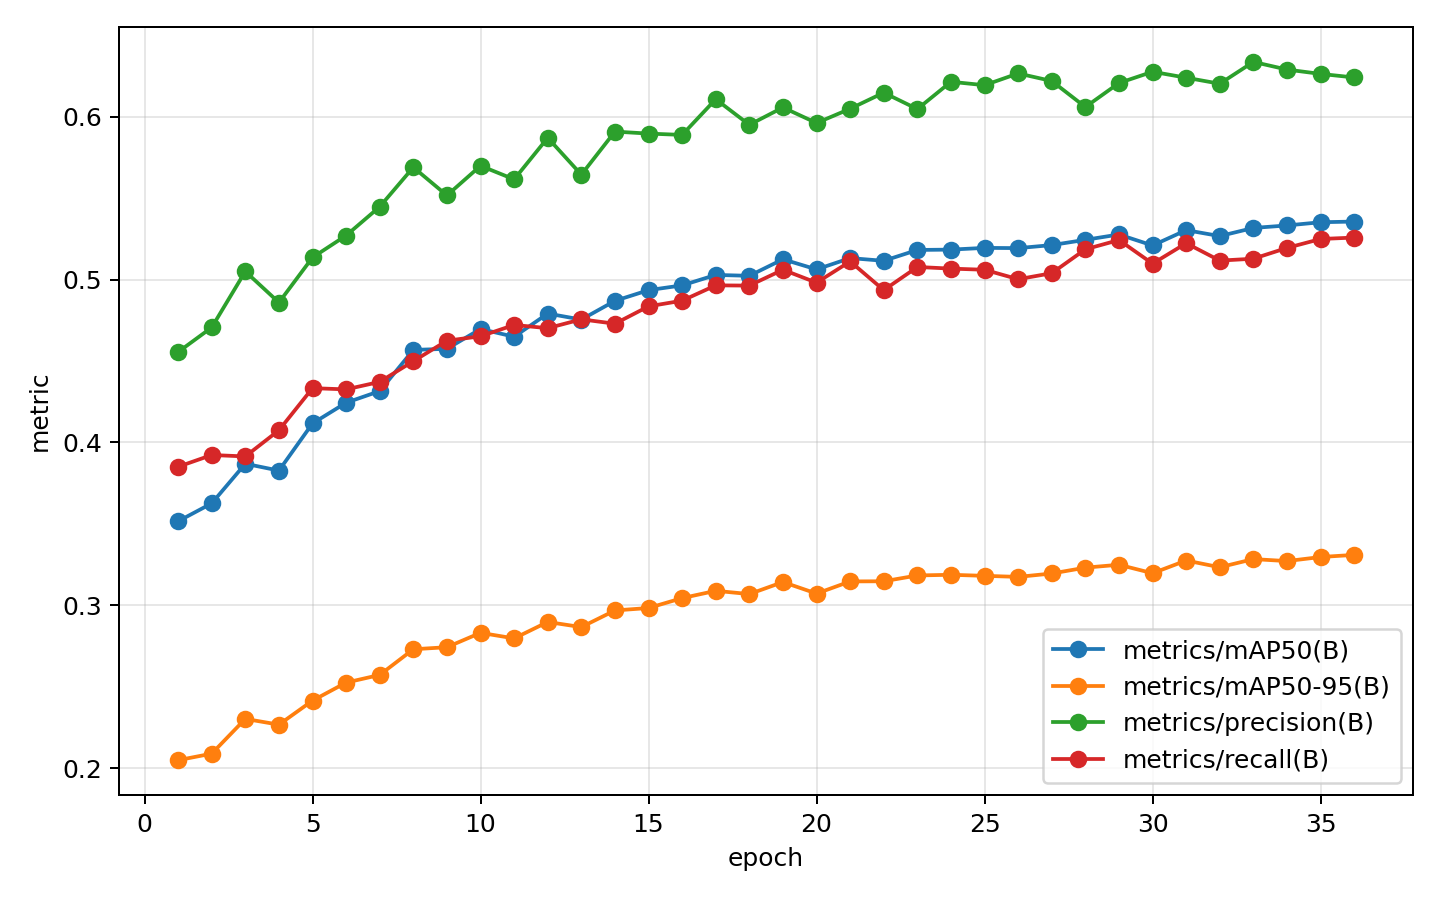
\includegraphics[width=\textwidth,height=0.3\textheight,keepaspectratio]{assets/detection_yolo11m_metrics.png}
      \vspace{0.2em}
      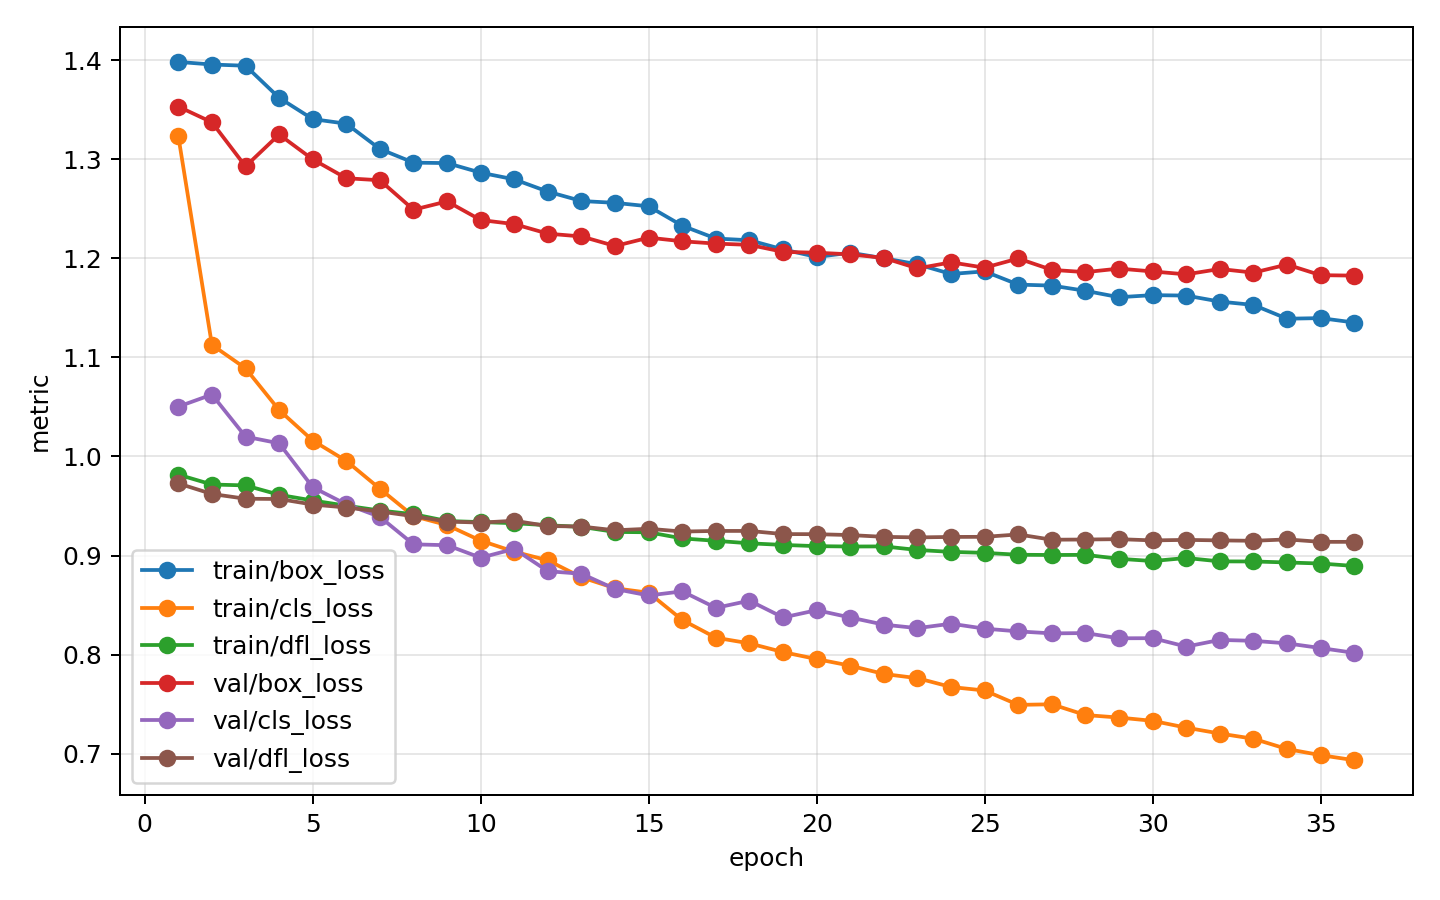
\includegraphics[width=\textwidth,height=0.3\textheight,keepaspectratio]{assets/detection_yolo11m_losses.png}
    \end{column}
  \end{columns}
\end{frame}

\begin{frame}{Tracking and Line-Crossing Algorithm}
  \centering
  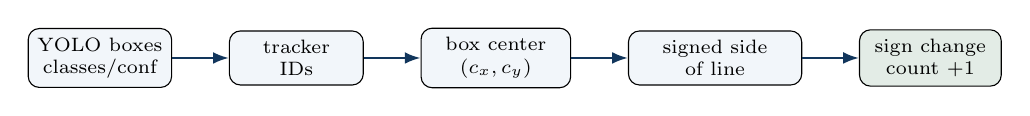
\begin{tikzpicture}[node distance=0.72cm]
    \node[box, minimum width=1.7cm] (boxes) {YOLO boxes\\classes/conf};
    \node[box, minimum width=1.7cm, right=of boxes] (track) {tracker\\IDs};
    \node[box, minimum width=1.9cm, right=of track] (center) {box center\\$(c_x,c_y)$};
    \node[box, minimum width=2.2cm, right=of center] (side) {signed side\\of line};
    \node[outbox, minimum width=1.8cm, right=of side] (count) {sign change\\count +1};
    \draw[arrow] (boxes) -- (track);
    \draw[arrow] (track) -- (center);
    \draw[arrow] (center) -- (side);
    \draw[arrow] (side) -- (count);
  \end{tikzpicture}
  \vspace{0.8em}
  \begin{block}{Counting rule}
    For each track ID, store which side of the line its center lies on. If the signed side changes sign and the ID has not been counted before, it is counted as one crossing.
  \end{block}
\end{frame}

\begin{frame}{Tracking Demo}
  \begin{columns}[T]
    \begin{column}{0.55\textwidth}
      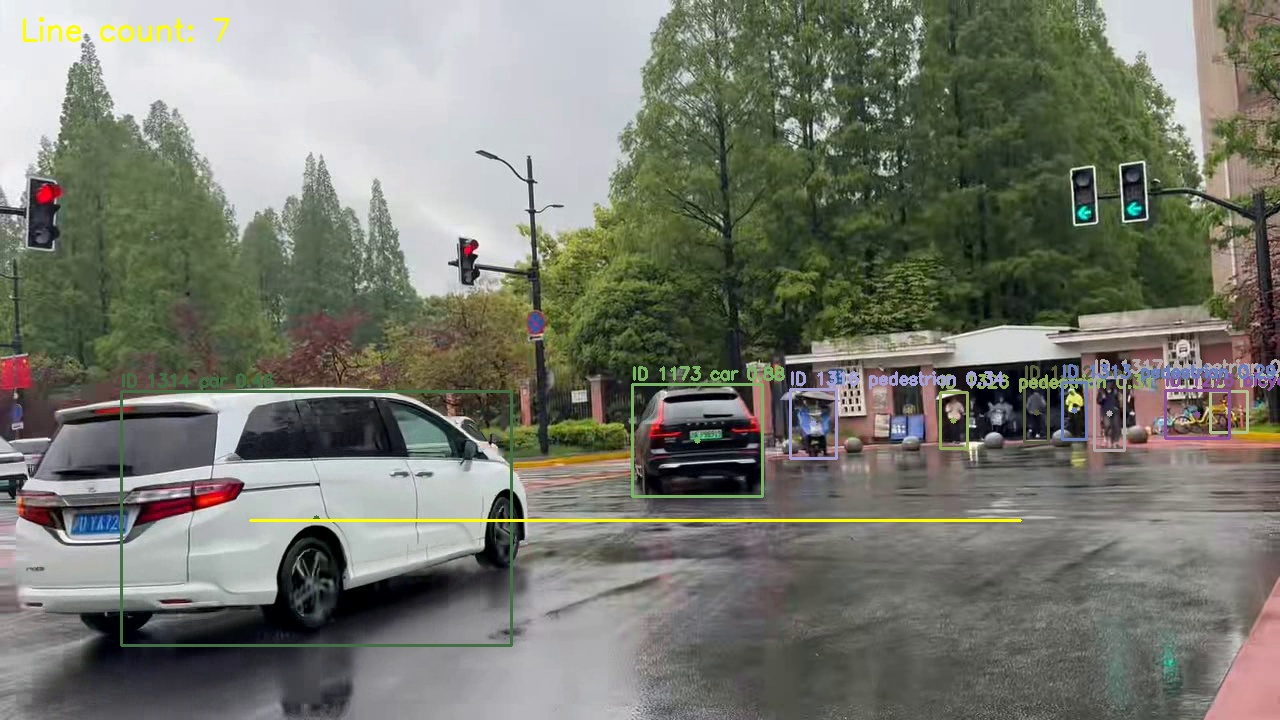
\includegraphics[width=\textwidth]{assets/tracking_counting_example_815.jpg}
    \end{column}
    \begin{column}{0.41\textwidth}
      \begin{block}{Demo file}
        {\scriptsize \texttt{presentation/videos/}\\\texttt{yolo11m\_bytetrack\_c025.mp4}}
      \end{block}
      \begin{itemize}
        \item YOLO11m detects boxes.
        \item ByteTrack maintains object IDs.
        \item Confidence threshold changes which objects survive into tracking.
      \end{itemize}
      \begin{block}{Fallback}
        The static frame shows IDs, line, and count if the video player fails.
      \end{block}
    \end{column}
  \end{columns}
\end{frame}

\begin{frame}{Overall Discussion}
  \begin{table}
    \centering
    \small
    \begin{tabular}{lll}
      \toprule
      Task & Bottleneck & What worked\\
      \midrule
      Classification & fine-grained representation & ImageNet pretraining + ResNet-34\\
      Segmentation & region overlap + boundary quality & Dice loss, but not Focal Loss\\
      Detection & tiny dense objects & YOLO11m + 960 input\\
      Tracking & ID stability under occlusion & lower-conf ByteTrack was more complete\\
      \bottomrule
    \end{tabular}
  \end{table}
  \begin{block}{Negative results}
    Random initialization, SE attention, Focal Loss, and high tracking confidence are useful because they show what did not match the main bottleneck.
  \end{block}
\end{frame}

\begin{frame}{Conclusion}
  \begin{itemize}
    \item The project completed all three required tasks plus controlled extension studies.
    \item The best models were selected by validation metrics and tested from best checkpoints.
    \item Final results: 90.60\% classification accuracy, 77.90\% segmentation mIoU, and 0.3310 detection mAP50-95.
    \item Code, configs, report, and weights are released through GitHub and ModelScope.
  \end{itemize}
  \vspace{0.6em}
  \begin{block}{Final message}
    A modification is useful only when it matches the real bottleneck of the task.
  \end{block}
\end{frame}

\begin{frame}{Appendix: Links and Backup}
  \begin{itemize}
    \item GitHub: \url{https://github.com/yuheng-li-ai/CV_Midterm}
    \item ModelScope weights: \url{https://www.modelscope.cn/models/yuhengli/cv-hw2-final-model}
    \item YOLO11 documentation: \url{https://docs.ultralytics.com/models/yolo11/}
    \item Tracking video: \texttt{presentation/videos/yolo11m\_bytetrack\_c025.mp4}
  \end{itemize}
  \begin{block}{Backup answer}
    YOLO11m@960 was stopped at epoch 36 due to deadline constraints, but it already had the strongest validation score among all detection runs.
  \end{block}
\end{frame}

\end{document}
